%%%%%%%%%%%%%%%%%%%%%%%%%%%%%%%%%%%%%%%%%%%%%%%%%%%%%%%%%%
%
% Vzor pro sazbu kvalifikační práce
%
% Západočeská univerzita v Plzni
% Fakulta aplikovaných věd
% Katedra informatiky a výpočetní techniky
%
% Petr Lobaz, lobaz@kiv.zcu.cz, 2016/03/14
%
%%%%%%%%%%%%%%%%%%%%%%%%%%%%%%%%%%%%%%%%%%%%%%%%%%%%%%%%%%

% Možné jazyky práce: czech, english
% Možné typy práce: BP (bakalářská), DP (diplomová)
\documentclass[czech,DP]{thesiskiv}

% Definujte údaje pro vstupní strany
%
% Jméno a příjmení; kvůli textu prohlášení určete, 
% zda jde o mužské, nebo ženské jméno.
\author{Zdeněk Valeš}
\declarationmale

%alternativa: 
%\declarationfemale

% Název práce
\title{Určování nahraditelnosti a\\kompatibility webových služeba}

% 
% Texty abstraktů (anglicky, česky)
%
\abstracttexten{The text of the abstract (in English). It contains the English translation of the thesis title and a short description of the thesis.}

\abstracttextcz{Text abstraktu (česky). Obsahuje krátkou anotaci (cca 10 řádek) v češtině. Budete ji potřebovat i při vyplňování údajů o bakalářské práci ve STAGu. Český i anglický abstrakt by měly být na stejné stránce a měly by si obsahem co možná nejvíce odpovídat (samozřejmě není možný doslovný překlad!).
}

% Na titulní stranu a do textu prohlášení se automaticky vkládá 
% aktuální rok, resp. datum. Můžete je změnit:
%\titlepageyear{2016}
%\declarationdate{1. března 2016}

% Ve zvláštních případech je možné ovlivnit i ostatní texty:
%
%\university{Západočeská univerzita v Plzni}
%\faculty{Fakulta aplikovaných věd}
%\department{Katedra informatiky a výpočetní techniky}
%\subject{Bakalářská práce}
%\titlepagetown{Plzeň}
%\declarationtown{Plzni}

%%%%%%%%%%%%%%%%%%%%%%%%%%%%%%%%%%%%%%%%%%%%%%%%%%%%%%%%%%
%
% DODATEČNÉ BALÍČKY PRO SAZBU
% Jejich užívání či neužívání záleží na libovůli autora 
% práce
%
%%%%%%%%%%%%%%%%%%%%%%%%%%%%%%%%%%%%%%%%%%%%%%%%%%%%%%%%%%

% Zařadit literaturu do obsahu
\usepackage[nottoc,notlot,notlof]{tocbibind}

% Umožňuje vkládání obrázků
\usepackage[pdftex]{graphicx}
\graphicspath{{./img/}}

% Odkazy v PDF jsou aktivní; navíc se automaticky vkládá
% balíček 'url', který umožňuje např. dělení slov
% uvnitř URL
\usepackage[pdftex]{hyperref}
\hypersetup{colorlinks=true,
  unicode=true,
  linkcolor=black,
  citecolor=black,
  urlcolor=black,
  bookmarksopen=true}

% Při používání citačního stylu csplainnatkiv
% (odvozen z csplainnat, http://repo.or.cz/w/csplainnat.git)
% lze snadno modifikovat vzhled citací v textu
\usepackage[numbers,sort&compress]{natbib}
%%%%%%%%%%%%%%%%%%%%%%%%%%%%%%%%%%%%%%%%%%%%%%%%%%%%%%%%%%
%
% VLASTNÍ TEXT PRÁCE
%
%%%%%%%%%%%%%%%%%%%%%%%%%%%%%%%%%%%%%%%%%%%%%%%%%%%%%%%%%%
\begin{document}
%
\maketitle
\tableofcontents

\chapter{Úvod}

- k čemu je práce dobrá
- co text práce obahuje
- use casy

\chapter{Principy webových služeb, techniky}

 - co je to API
 - co jsou to webové služby
 - REST

\chapter{Datové typy a porovnávání}

- přednášky FJP
- jak jazyky řeší datové typy
- tady budu citovat \cite{abadi1995subytping}
	- subtyping
	- kontrvaariance


\chapter{Popis ukládání metadat v CRCE, popis indexování API}

\section{Metadata v CRCE}

 - tady budu citovat \cite{brada2015repository}
 - Resource + Capability
 - Capability mají Attributy + Properties
 - Properties mají atributy
 
 \begin{figure}[h]
 	\centering
 	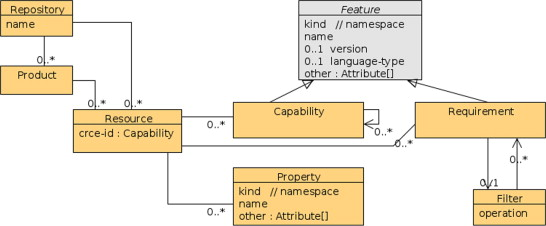
\includegraphics{resource-uml}
 	\caption{Reprezentace metadat v CRCE}
 	\label{fig:crce-resource-uml}
 \end{figure}

\section{Indexování API}

- různé druhy jsou jinak indexované
- každý druh API indexován vlastním modulem
- popis opravených chyb
- taky budu citovat diplomky od Pejřimovského \cite{pejrimovsky2015ws} a Hessové \cite{hessova2015rest}

\chapter{Popis funkce porovnávače (co se jak porovnává pro jaké typy API)}

- zmínit taky omezení, která plynou z indexovaných dat
- v podstatě se porovnávají stromy Capabilit
- detaily v euromicro článku
- popsat MOV


\chapter{Implementační detaily (jen stručně)}


\chapter{Testování}

- nějaká reálná data
	- STAG (WSDL)
- i syntetická data
 
% 
% PRO ANGLICKOU SAZBU JE NUTNÉ ZMĚNIT
% CITAČNÍ STYL!
%
\bibliographystyle{csplainnatkiv}
{\raggedright\small
\bibliography{literatura}
}

\end{document}
